\documentclass[8pt,notitlepage,fleqn]{extarticle}
\usepackage[letterpaper,margin=0.25in,heightrounded]{geometry}
\usepackage{mathtools,amssymb,amsfonts,amsthm,empheq,mdframed,booktabs}
\allowdisplaybreaks[1]
\usepackage{tikz}
\usetikzlibrary{arrows.meta,calc,decorations,shapes.geometric}
%\usepackage{pgfplots}

\usepackage[T1]{fontenc}
\usepackage{lmodern}   % scalable fonts
\usepackage{microtype}
\usepackage{titlesec}
\titlespacing{\section}{0pt}{0pt}{0pt}

\usepackage{multicol}
\usepackage{siunitx}
\usepackage[version=4]{mhchem}

\title{Modern Physics Reference Sheet --- Ch. 38,39}
\author{Miraj Parikh \hfill Jie --- 2}
\date{2025 October}

% custom title
\makeatletter
\renewcommand*{\maketitle}{%
\noindent
\hfill
\begin{minipage}{0.75\textwidth-2pt}
\begin{tikzpicture}
\node[rectangle,rounded corners=6pt,inner sep=10pt,fill=blue!50!black,text width= 0.95\textwidth] {\color{white}\huge \@title};
\end{tikzpicture}
\end{minipage}
\begin{minipage}{0.25\textwidth-2pt}
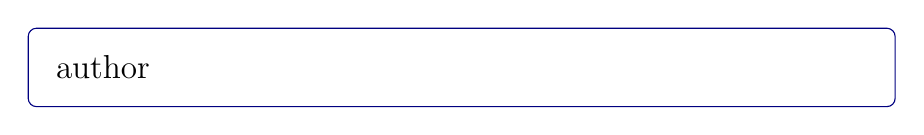
\begin{tikzpicture}
\node[rectangle,rounded corners=3pt,inner sep=10pt,draw=blue!50!black,text width= 0.85\textwidth] {\large \@author};
\end{tikzpicture}
\end{minipage}
\hfill
\bigskip
}%
\makeatother

\let\vec\mathbf

\begin{document}
\fontsize{6}{2}\selectfont

  \thispagestyle{empty}
  \maketitle
  \begin{multicols*}{2}
  \setlength{\mathindent}{0pt}
  \setlength{\columnsep}{10pt}
  \setlength{\parskip}{0pt}
  \setlength{\jot}{2pt}
  \setlength{\abovedisplayskip}{2pt}
  \setlength{\abovedisplayshortskip}{2pt}
  \setlength{\belowdisplayskip}{2pt}
  \setlength{\belowdisplayshortskip}{2pt}
  \raggedcolumns
  \section*{Constants}
  \begin{gather}
    c = \lambda \nu = \qty{2.997925e8}{\meter\per\second} \tag{Speed of Light} \\
    e = q_e = q_p = \qty{1.602177e-19}{\coulomb} \implies \qty{1}{\electronvolt} = \qty{1.602177e-19}{\joule} \tag{Unit Charge} \\
    k_\mathrm{e} = \qty{8.987551e9}{\newton\meter\squared\per\coulomb\squared} \tag{Coulomb Constant} \\
    \varepsilon_0 = \qty{8.854188e-12}{\coulomb\squared\per\newton\per\meter\squared} \tag{Permittivity of Free Space} \\
    m_e = \qty{9.109384e-31}{\kilogram} \tag{Electron Mass} \\
    m_p = \qty{1.672622e-27}{\kilogram} \tag{Proton Mass} \\
    h = \qty{6.626070e-34}{\joule\second} = \qty{4.135668e-15}{\electronvolt\second} \tag{Planck Constant} \\
    \hbar = h/2\pi = \qty{1.054572e-34}{\joule\second} = \qty{6.582120e-16}{\electronvolt\second} \tag{Reduced Planck Constant} \\
    R_{\ce{H}} = \qty{1.097373e7}{\per\meter} \tag{Rydberg Constant of an \ce{H} Atom} \\
    % k_B = \qty{1.380649e-23}{\joule\per\kelvin} = \qty{8.617333e-5}{\electronvolt\per\kelvin} \\
    % \mu_0 = 4\pi\times\qty{e-7}{\newton\per\ampere\squared} \\
    hc = \qty{1.986446e-25}{\joule\meter} = \qty{1.239842e-6}{\electronvolt\meter} \tag{Product of \(h\) and \(c\)} \\
    E_1 = \qty{13.59844}{\electronvolt} \tag{Total Mechanical Energy of a Ground-State Electron of a \ce{H} atom} \\
    \lambda_\mathrm{C} = h/m_ec = \qty{2.426310e-12}{\meter} \tag{Compton Wavelength}
  \end{gather}
  \section*{Formulae and Equations}
  \subsection{Relativity}
  \begin{gather}
    \beta \coloneq v/c \tag{Definition of Fraction of Speed of Light} \\
    \gamma \coloneq 1/\sqrt{1-(v/c)^2} = 1/\sqrt{1-\beta^2} \tag{Definition of Lorentz Factor} \\
    s^2 = (c\Delta t)^2 - (\Delta \vec{x})^2 \implies \mathrm{d}S = (c\mathrm{d}t)^2 - (\mathrm{d}\vec{x})^2 \tag{Spacetime Interval} \\
    L_\text{obs} = L_\text{real}/\gamma \tag{Length Contraction} \\ 
    t_\text{obs} = t_\text{real}\gamma \tag{Time Dilation}
  \end{gather}
  \subsection{Particle Variables}
  \begin{gather}
    E = h\nu = hc/\lambda \tag{Planck relation} \\
    \lambda = h/p = h/mv \implies p = E/c = h/\lambda \tag{De Broglie Wavelength}
  \end{gather}
  \subsubsection{Quantized Particle Model}
  \begin{gather}
    E = nh\nu = nhc/\lambda \tag{Quantized Planck relation} \\
    \Delta \lambda = h/m_ec\left(1-\cos{\theta}\right) = \lambda_\mathrm{C}\left(1-\cos{\theta}\right) \tag{Compton Scattering}
  \end{gather}
  \subsubsection{Electrons}
  Properties of photoelectrons from metal with work function \(W\):
  \begin{gather}  
    E_\mathrm{\gamma} = W + K_{e^-\mathrm{(max)}} \implies K_{e^-\mathrm{(max)}} = h\nu - W = h(\nu-\nu_0) \tag{Conservation of Energy} \\
    eV_S \coloneq K_{e^-\mathrm{(max)}} \implies V_S = h/e\left(\nu-\nu_{0}\right) \tag{Definition of Stopping Potential}
  \end{gather}
  Properties of the electron in a \(Z\)-hydrogenic atom of principal quantum number \(n\):
  \begin{gather}
    2\pi r_n = \lambda n \implies L_n = m_ev_nr_n = n\hbar \tag{Bohr Model; Angular Momentum} \\
    F_c = \frac{mv^2}{r} = \frac{m_ev_n^2}{r_n} \tag{Centripetal Force} \\
    F_\mathrm{e} = k_\mathrm{e}\frac{q_1q_2}{r^2} = k_\mathrm{e}\frac{(e)(Ze)}{r_n^2} = \frac{1}{4\pi\varepsilon_0}\frac{Ze^2}{r_n^2} = k_\mathrm{e}\frac{Ze^2}{r_n^2} \tag{Electrostatic Force} \\
    F_\mathrm{e} = F_c \implies v_n^2r_n = k_\mathrm{e}\frac{Ze^2}{m_e} \tag{Electrostatic Force functioning as Centripetal Force} \\
    v_n = \left(m_e \cdot v_n^2r_n\right) / \left(m_ev_nr_n\right) = \frac{k_\mathrm{e} Ze^2}{n\hbar} \tag{Orbital Velocity} \\
    r_n = \left(m_ev_nr_n\right) / \left(m_e \cdot v_n\right) = \frac{n^2\hbar^2}{m_ek_\mathrm{e}Ze^2} = a_0\frac{n^2}{Z} \tag{Orbital} \\
    a_0 \coloneq \frac{\hbar^2}{m_ek_\mathrm{e} e^2} = \frac{4\pi\varepsilon_0\hbar^2}{m_e e^2} = \frac{\varepsilon_0 h^2}{\pi m_e e^2} \tag{Definition of Bohr Radius} \\
    U_n = -k_\mathrm{e}\frac{q_1q_2}{r} = -k_\mathrm{e}\frac{(e)(Ze)}{r_n} = -\frac{k_\mathrm{e} Z e^2}{r_n} = -\frac{k_\mathrm{e}^2 Z^2 m_e e^4}{n^2\hbar^2} \tag{Potential Energy}\\
    K_n = \frac{1}{2}mv^2 = \frac{1}{2}m_ev_n^2 = \frac{k_\mathrm{e}^2Z^2m_ee^4}{2n^2\hbar^2} \implies 2K_n + U_n = 0\tag{Kinetic Energy}\\
    E_n = K_n + U_n = -\frac{k_\mathrm{e}^2Z^2m_ee^4}{2n^2\hbar^2} = -E_1\frac{Z^2}{n^2} \tag{Total Mechanical Energy Magnitude} \\
    E_1 \coloneq \frac{k_\mathrm{e}^2m_ee^4}{2\hbar^2} = \frac{m_e e^4}{8\varepsilon_0h^2}\tag{Total Mechanical Energy Magnitude for \(n=1\) \ce{H} Electron} \\
    \frac{1}{\lambda} = R_{\ce{H}} \left( \frac{1}{n_1^2} - \frac{1}{n_2^2} \right) \tag{Rydberg Formula} \\
    R_{\ce{H}} \coloneq -\frac{m_e e^4}{8h^3\varepsilon_0^3c}\tag{Rydberg Formulae for a \ce{H} Electron}
  \end{gather}
  Note: \(a_0\) also equals the modal distance between the nucleus and electron of a \ce{H} atom.
  Note: Velocities are assumed to be non-relativistic (\(v \ll c\)).
  \subsection{Sinusoidal Waves}
  \(T\) is to \(\omega\) as \(\lambda\) is to \(k\).
  Note: \(\varphi\), phase shift, will vary between different expressions of \(D\) where initial conditions like \(x_{0}\) and \(t_{0}\) are set. Note: \textbf{SWD} refers to the formula of sinusoidal wave spatial–temporal displacement, \(D(x,t)\).
  \begin{gather}
    f \coloneq 1/T \implies T = 1/f, fT = 1 \tag{Definition of Frequency} \\
    \omega \coloneq 2\pi / T \implies \omega = 2\pi f, T = 2\pi/\omega, f = \omega / 2\pi \tag{Defintion of Angular Frequency}\\
    \lambda \coloneq v / f \implies v = \lambda f = \lambda / T, vT = \lambda \tag{Definition of Wavelength}\\
    k \coloneq 2\pi / \lambda \implies v = \omega / k \tag{Definition of Wavenumber}\\
    D(x,t) = A\sin{\left(2\pi\left(\frac{x}{\lambda} - \frac{t}{T}\right) + \varphi\right)} = A\sin{\left(kx - \omega t + \varphi\right)} \tag{SWD} \\ 
    D(x,t) = A\sin{\left(\frac{2\pi}{\lambda}\left(x - vt\right) + \varphi\right)} \tag{SWD parametrized to \(x-vt\)} \\ 
    D(x,t_0) = A\sin{\left(2\pi \frac{x}{\lambda} + \varphi'\right)} = A\sin{\left(kx + \varphi'\right)} \tag{SWD in a Snapshot Graph} \\ 
    D(x_0,t) = A\sin{\left(-2\pi ft + \varphi'\right)} = A\sin{\left(-\omega t + \varphi'\right)} \tag{SWD in a History Graph} \\
    D(x, t) = D(x + n\lambda, t + mT) \; \forall\, n, m \in \mathbb{Z} \tag{SWD spatial-temporal periodicity} \\
    V(x, t) = \frac{{\partial}D(x,t)}{{\partial}t} = -\omega A \cos{\left(kx - \omega t + \varphi\right)} \tag{SWD particle velocity} \\
    V(x_0, t) = \left.{\frac{{\partial}D(x,t)}{{\partial}t}}\right\vert_{x=x_0} = -\omega A \cos{\left(\omega t + \varphi'\right)} \tag{SWD particle velocity history graph}
  \end{gather}
  \subsection{Quantum Mechanics}
  \subsubsection{Schrödinger's Equation}
  \begin{equation}
  \hat{H}\langle\Psi(t)| = i\hbar \frac{\mathrm{d}}{\mathrm{d}t} \langle\Psi(t)| \implies -\frac{\hbar^2}{2m}\nabla^2\Psi + V(\vec{x})\Psi = i\hbar\frac{{\partial}\Psi}{{\partial}t} \tag{Time-dependent}
  \end{equation}
  \begin{equation}\hat{H}\langle\Psi| = E\langle\Psi| \implies -\frac{\hbar^2}{2m}\nabla^2\Psi + V(\vec{x})\Psi = E\Psi \tag{Time-independent}\end{equation}
  % One-dimensional, time-dependent: \begin{equation*}-\frac{\hbar^2}{2m}\frac{{\partial}^2\Psi}{{\partial}x^2} + V(x)\Psi = i\hbar\frac{{\partial}\Psi}{{\partial}t}\end{equation*}
  % One-dimensional, time-independent: \begin{equation*}-\frac{\hbar^2}{2m}\frac{{d}^2\Psi}{{d}x^2} + V(x)\Psi = E\Psi\end{equation*}
  \end{multicols*}
\end{document}
